\begin{figure}[t]
	\label{fig_method}
	\centering
	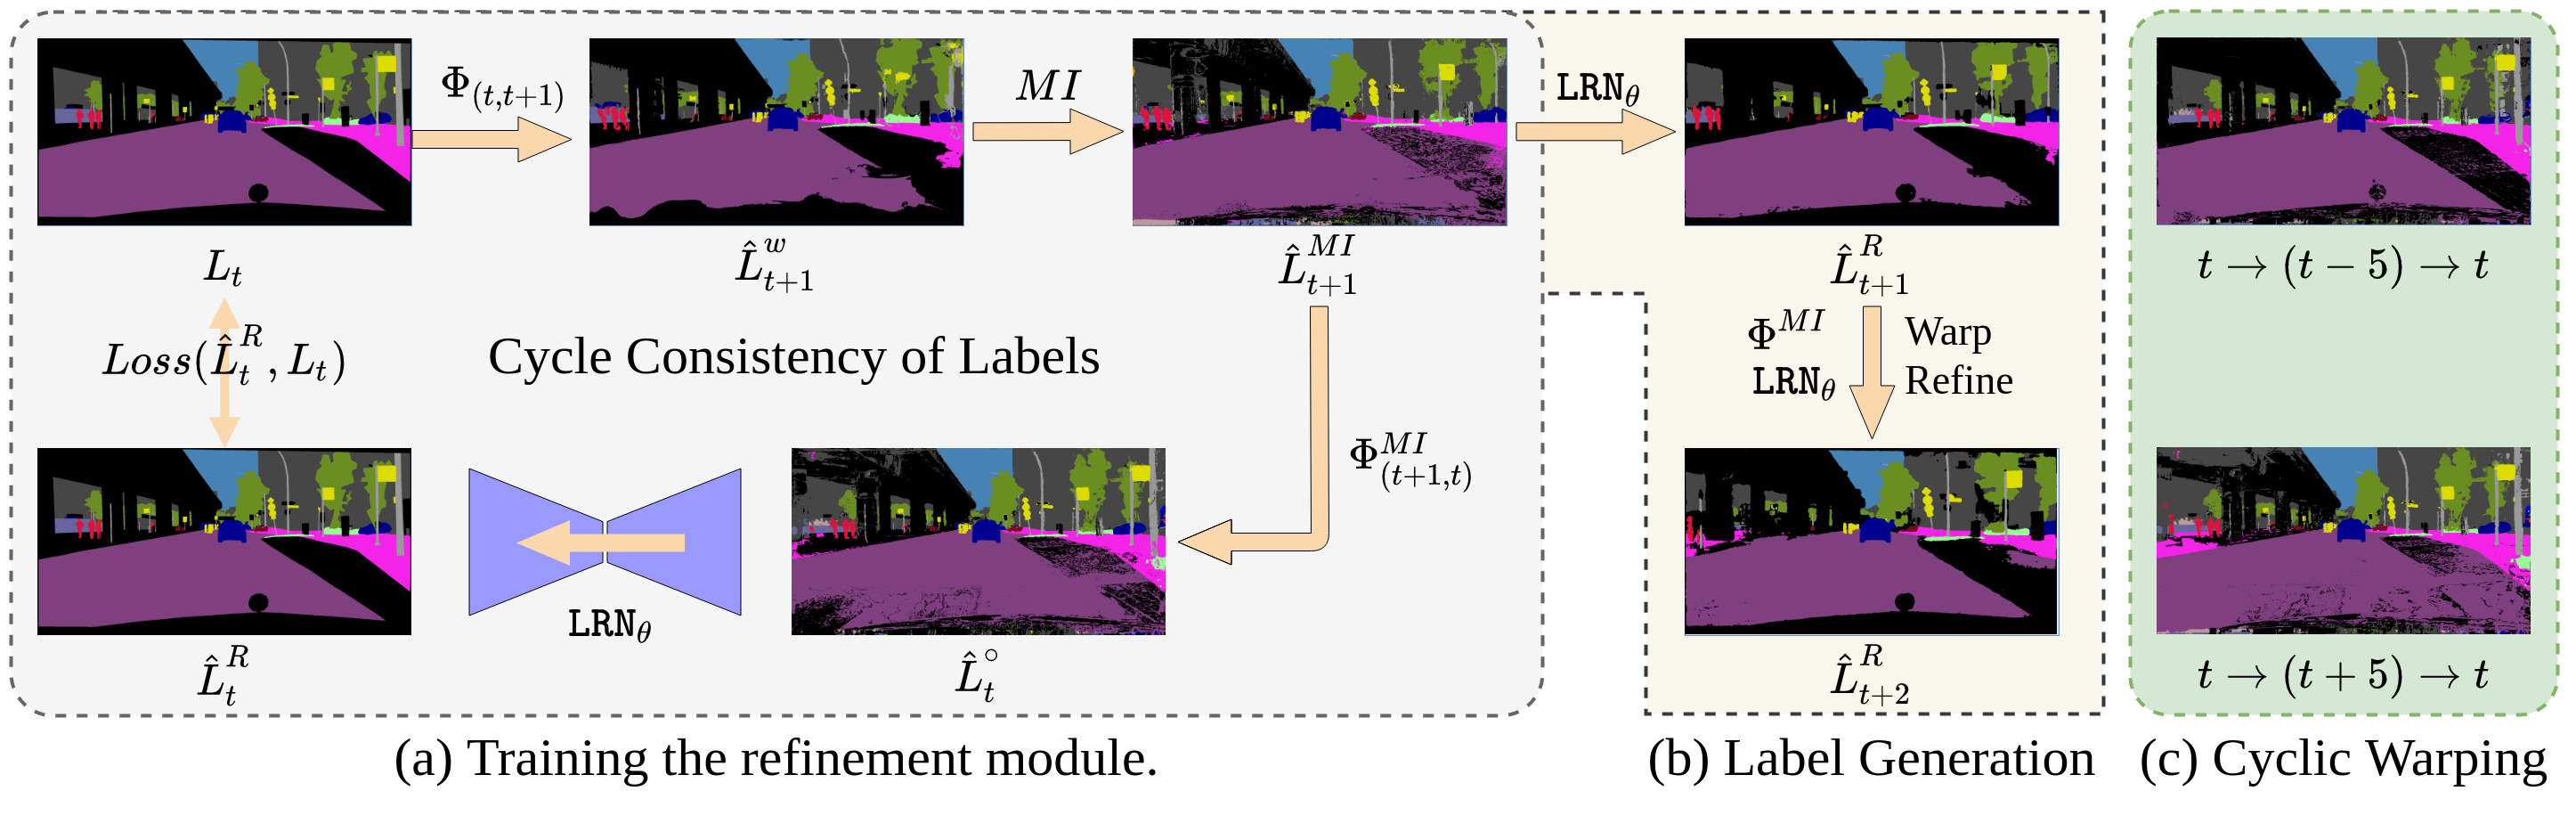
\includegraphics[width=1.0\linewidth]{figures/process_smaller_lr.png}
    \vspace{-2em}
	\caption{\small (a) For training $\texttt{LRN}_\theta$, the cyclic propagated labels $\hat{L}^{\circ}$ are used as input, as given by equation~\eqref{eq-cyclic-process}. (b) While generating labels, the warped post-processed labels $\hat{L}^{MI}$ are given as input to $\texttt{LRN}_\theta$. Iterative application of warping and refining is used to generate sequential labels. (c) The cyclic warped labels are generated for a wider range of cyclic loops to expose $\texttt{LRN}_\theta$ to more warping error while training.}
    \vspace{-1em}
\end{figure}
